\documentclass[12pt]{article}

\usepackage[dvips,letterpaper,margin=0.75in,bottom=0.5in]{geometry}
\usepackage{cite}
\usepackage{slashed}
\usepackage{graphicx}
\usepackage{amsmath}
\usepackage{amssymb}
\usepackage{braket}
\usepackage{pythonhighlight}
\usepackage{mathtools}
\usepackage{tikz}
\usepackage{bm}
\usepackage{hyperref}
\usepackage{microtype}
\usepackage{geometry}

\begin{document}

\title{PHY 112L \\ Ising Model}
\author{Michael Mulhearn}

\maketitle

\section{Introduction}

In this assignment, you will simulate phase transitions in a
ferromagnetic material by applying the Metropolis-Hastings algorithm to
the Ising model.

\section{The Metropolis-Hastings Algorithm}

A discrete-time Markov Chain is a countably infinite sequence of
random variables:
$$X_1, X_2, X_3, \ldots, X_n, X_{n+1}, \ldots$$
where the probability of outcome $X_{n+1}$ depends {\em solely} on
outcome $X_{n}$.  We can write this requirement formally as:
$$Pr(X_{n+1} | X_1, X_2, \ldots, X_{n}) = Pr(X_{n+1}| X_n)$$ The
indices are generally interpreted as time steps, and the change from
$X_n$ to $X_{n+1}$, following $Pr(X_{n+1}|X_{n}$), is called a {\bf
  transition}. 

The memory-less nature of a Markov Chain makes it quite well suited for
use in computer simulations, which then need only track the current
state, compute the transition, and update the current state.  The
Metropolis-Hastings (MH) Algorithm is a widely used example of a
Markov chain Monte Carlo method of computer simulation.  We are using
large $X$ here as a reminder that $X$ need not be a simple variable
(like a single integer or real number).  For example, in our case, $X$
will be an $L \times L$-sized array of integers.  $X$ can be quite
large, and it is therefore a major advantage that we need only store
one value of $X$ in computer memory.

The MH algorithm obtains random variables of a desired probability
distribution $p(X)$ by constructing a Markov Chain, using only
knowledge of some function $f(X)$ that is proportional to $p(X)$.  This
is a considerable simplification, as the normalization may be
difficult or even impossible to calculate.  For example, in our
application of this algorithm to statistical mechanics, we will use
the Boltzmann factor, but we will not need to determine the partition
function.

In the MH algorithm, the Markov Chain is constructed using a propose
and accept approach.  For the proposal, starting from the current
state $X$, we propose an updated state $Y$, according to probability
$Q(X \to Y)$.  In our case, we will design the proposals to be
symmetric, so that:
\begin{equation}
\label{eqn:symmetric}
Q(X \to Y) = Q(Y \to X)
\end{equation}
Next, we accept the new state $Y$ with
probability $A(X \to Y)$.  If we do not accept the new state, we
simply hold the current state for the next step as well.
By construction, the probability that a state $X$ is updated to a new
state $Y \ne X$ is therefore:
$$W(X \to Y) = Q(X \to Y) A(A \to Y)$$

So far, we have only succeeded in constructing a Markov Chain.  But we
want to construct the specific Markov chain whose elements $X$, after
many updates, approach the desired probability distribution $p(X)$.
A sufficient condition is to impose {\bf
  detailed balance}:
\begin{equation}
p(X) W(X \to Y) = p(Y) W(Y \to X)
\end{equation}
Or equivalently:
\begin{eqnarray*}
 \frac{p(Y)}{p(X)} &=& \frac{W(X \to Y)}{W(Y \to X)} \\
                   &=& \frac{Q(X \to Y)}{Q(Y \to X)} \frac{A(X \to Y)}{A(Y \to X)} \\
                   &=& \frac{A(X \to Y)}{A(Y \to X)} \\
\end{eqnarray*}
For a system in thermal equilibrium at temperature $T$, we expect that
the probability of each microstate is proportional to a Boltzmann factor,
so that:
\begin{equation}
\label{eqn:boltzmann-balance}
  \frac{p(Y)}{p(X)} = \exp\left( -\frac{E_Y - E_X}{kT} \right)
\end{equation}
where $E_X$ and $E_Y$ are the total energy of the microstates $X$ and $Y$.
We therefore define the acceptance probability for a transition from $X$ to $Y$ as follows:
\begin{equation}
  A(X \to Y) =
  \begin{cases}
    1 & E_Y < E_X \\[4pt]
    \displaystyle \exp\left( -\frac{E_Y - E_X}{kT} \right) & {\rm otherwise} \\
  \end{cases}
\end{equation}
which ensures that:
$$0 \leq A(X \to Y) \leq 1$$
and Equation~\ref{eqn:boltzmann-balance} is satisfied (which you
should verify for yourself by carefully working it through explicitly
for both $E_Y > E_X$ and $E_Y < E_X$.)

\section{The Ising Model}

The Ising model is a beguilingly simple yet phenomenologically rich
model for ferromagnetism.  In two dimensions, it already exhibits a
realistic phase transition.  It is also ideally suited to numerical
simulation with the MH algorithm.

In 2-D, the material is modeled as an $L \times L$ lattice of atomic
spins, $s_i$, which are each either up ($s_i=1$) or down ($s_i=-1$).
Each spin has a magnetic dipole moment that is assumed to influence
only its nearest neighbors.  In the absence of an external magnetic
field, the total energy for the entire lattice is given by the
Ising-model Hamiltonian
\begin{equation}
H = - J \sum_{\braket{i,j}} \, s_i \, s_j 
\end{equation}
where the sum over $\braket{i,j}$ is over pairs of nearest neighbors.
It is an easy mistake to double count nearest neighbors when
implementing the Ising model, so take care that if site A and site B
are nearest neighbors, they occur exactly once in the sum.  Notice
that for $J>0$ it is energetically favorable for neighboring spins to
align, and this is used to model ferromagnetic materials.

The magnetization per spin is:
\begin{equation}
  m \;=\; \frac{1}{L^2}\sum_i s_i
\end{equation}
and the energy per spin is:
\begin{equation}
  e \;=\; \frac{H}{L^2}
\end{equation}

Consider a single spin $s_i$.  The energy between this spin and its neighbors, when it is oriented upward is:
$$E_{\uparrow} = - J \sum_{j \; \in \; N(i)} \; s_j$$
where $N(i)$ is the set of neighboring spins of $i$. It follows that:
\begin{equation}
E_{\uparrow} = - J n \bar{s}
\end{equation}
where:
$$\bar{s} \equiv \frac{1}{n} \sum_{j \; \in \; N(i)} \; s_j $$
is the average alignment of the neighbors, and $n=4$ in our 2-D case.  When the spin is oriented downward we have:
\begin{equation}
E_{\downarrow} = J n \bar{s}
\end{equation}
The partition function for the single spin is then:
$$Z_i = exp(-Jn\bar{s}/kT) + exp(-Jn\bar{s}/kT) = 2 cosh(Jn\bar{s}/kT)$$
and the expected value for the spin is:
$$\bar{s_i} = \frac{(1)\,\exp(Jn\bar{s}/kT) + (-1)\,\exp(-Jn\bar{s}/kT)}{Z_i} = \frac{2 \sinh(Jn\bar{s}/kT)}{2 \cosh(Jn\bar{s}/kT)} = \tanh(Jn\bar{s}/kT)$$
In the mean field approximation, we assume that:
$$s_i = \bar{s}$$
that is, each spin is typical in the sense that it has the same
expected value as its neighbors.  And obtain:
\begin{equation}
\label{eqn:mfa}
\bar{s} = \tanh(Jn\bar{s}/kT)
\end{equation}

\begin{figure}[thb]
\begin{center}
{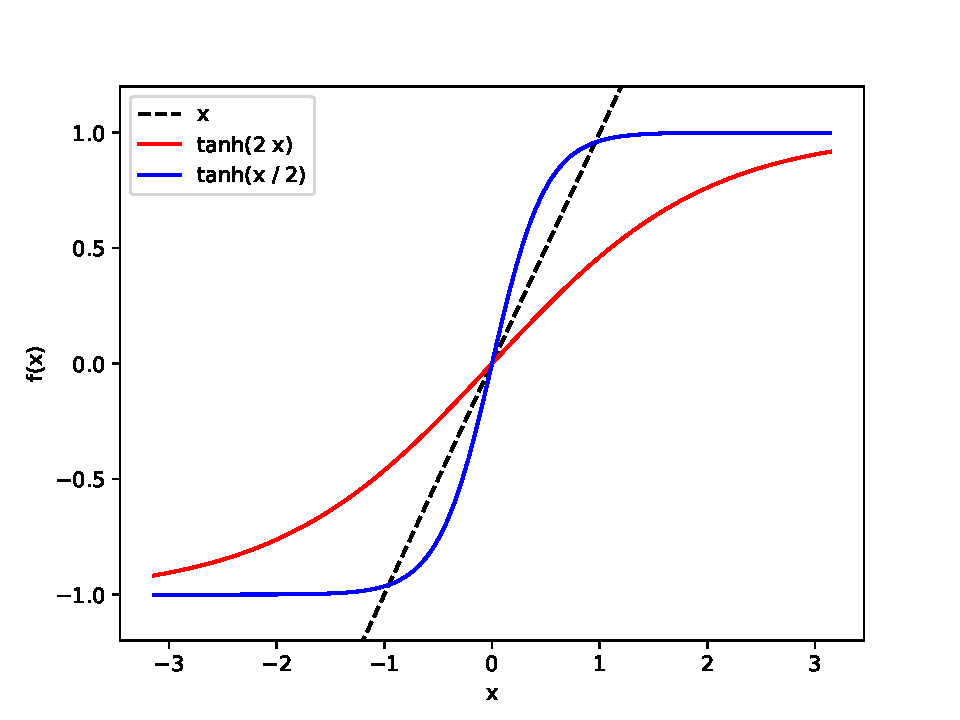
\includegraphics[width=0.60\textwidth]{plots/ssb.pdf}}
\end{center}
\caption{\label{fig:ssb} Spontaneous symmetry breaking in the Ising model under the mean field approximation.}
\end{figure}

As illustrated in Fig.~\ref{fig:ssb}, when $J n / k T < 1$, there is
only a single solution to Equation~\ref{eqn:mfa} at $\bar{s}=0$.
However, when $J n / k T > 1$ there are additional solutions at
positive and negative $\bar{s}$.  In this case, however, the solution
at $\bar{s}=0$ is unstable.  If a small fluctuation makes $\bar{s}$
non-zero, e.g. positive, then $\tanh(Jn\bar{s}/kT)$ is even more
positive.  

Below
\begin{equation}
T_{\rm C} = J n / k = 4 J / k
\end{equation}
the magnetization is zero, but above this
temperature, the magnetism takes some non-zero value.  This is an
excellent example of spontaneous symmetry breaking.  When observed,
the systems will tend to align upward or downward, seemingly
indicating a preferred direction, but in fact, the probability of the
system to point upward is equal to the probability it will point
downward, consistent with the symmetry of our system.

The exact solution for the Ising model for an infinite lattice is
\begin{equation}
T_{\rm C} \;=\; \frac{2J}{\ln(1+\sqrt{2})} \;\approx\; 2.269\,J
\end{equation}
We will model a finite lattice, with a slightly reduced critical temperature.


\section{System of Units}

We assume there is some temperature scale of interest $T_0$ and we define the unit of energy as:
$$\epsilon \equiv k T_0$$
Thus we can write the Hamiltonian as:
$$\frac{H}{\epsilon} = -\frac{J}{\epsilon} \sum_{\braket{i,j}} s_i s_j $$
and the critical temperature as:
$$\frac{T_{\rm C}}{T_0} = n \frac{J}{\epsilon}$$
As always, we set $T_0 = \epsilon = 1$ in our numerical code.

\section{Numerical Model for the Ising Model}

We will use \emph{periodic boundary conditions}.  This means every
site has exactly four neighbors (up, down, left, right), and indices
wrap modulo $L$.  Periodic boundaries reduce surface effects, which is
particularly important for small scale models such as ours.

\begin{itemize}

\item We initialize an $L \times L$ array with each value either 1 or -1.

\item We pick a randomly chosen site and flip its sign.  This is
  symmetric, so that Equation~\ref{eqn:symmetric} is satisfied.

\item Calculate the energy change $\Delta E$ due to the flip:
$$ \frac{\Delta E}{\epsilon} \;=\; 2 \frac{J}{\epsilon} s_i \sum_{\text{nn}} s_j $$
where $\sum_{\text{nn}}$ denotes the sum over the four nearest neighbors of site $i$.
  
\item If $\Delta E < 0$, accept the proposed flip. If not, accept the flip with probability
  $$p = \exp\left(-\frac{\Delta E}{\epsilon} \frac{T_0}{T} \right)$$

\end{itemize}





\section{Required Functions}

You must implement the following functions as part of your solution.
You may substitute similar signatures if using a language other than
Python, but you must use exactly these signatures if using Python. You
do not need to include the docstrings.  You are encouraged to define
additional functions as part of your solution, but these functions are
the most significant.

\begin{python}
def random_lattice(*, L):
    """
    Return an LxL 2-D lattice with randomly assigned spin values.

    Parameters:
      L : int 1-D   length of square lattice

    Returns:
      ndarray of int, shape (L, L) randomly filled with +1 or -1.
    """
    pass
\end{python}

\begin{python}
  def const_lattice(*, s, L):
    """
    Return an LxL 2-D lattice filled with a constant spin value.

    Parameters:
      s : int Spin value to assign to every lattice site 
      L : int 1-D   length of square lattice

    Returns:
      ndarray of int, shape (L, L) filled with value s.
    """
\end{python}

\begin{python}
def avg_energy(lattice, *, J=1.0):
    """
    Return the average energy per spin of a 2-D spin lattice.

    Parameters:
      lattice : ndarray of int, shape (L, L), spin configuration
      J : float coupling strength

    Returns:
      float total energy of the lattice configuration.
    """
    pass
\end{python}      

\begin{python}
def avg_magnetization(lattice):
    """
    Return the average magnetization per spin of a 2-D spin lattice.

    Parameters:
      lattice : ndarray of int, shape (L, L), spin configuration

    Returns:
      int absolute value of the total magnetization.
    """
\end{python}      

\begin{python}
def metropolis_flip(lattice, *, T, nsweep=1, J=1.0):
    """
    Update a 2-D spin lattice using the Metropolis algorithm.

    A total of nsweep x L x L single-spin flip attempts are made,
    where each attempt chooses a random lattice site and applies the
    Metropolis acceptance criterion.

    Parameters:
      lattice : ndarray of int, shape (L, L), spin configuration
      T : float temperature
      nsweep : int number of full-lattice sweeps
      J : float coupling strength

    Returns:
      ndarray of int, shape (L, L) updated lattice configuration.
    """
    pass  
\end{python}


\section{Homework Problems}

\noindent
{\bf Problem 1:} Implement the functions {\tt random\_lattice} and
{\tt constant\_lattice} and demonstrate that they work by printing the
lattice for a few different test cases.\\[4pt]

\noindent
{\bf Problem 2:} Implement the functions {\tt avg\_energy} and {\tt
  avg\_magnetization} and test that they give the expected results
for constant lattices of +1 and -1.\\[4pt]

\noindent
{\bf Problem 3:} Implement the function {\tt metropolis\_flip}.  For a
random lattice with $L=10$, $T=0.1~T_0$ and $J=1$, show that after {\tt
  nsweep=1000} the final state is either all 1's or all -1's.  This is
an example of spontaneous symmetry breaking.\\[4pt]

\noindent
{\bf Problem 4:} For each temperature $T$, initialize a random lattice
with $L=10$ and $J=1$, then apply {\tt NINIT=200} sweeps to initialize
the lattice.  Follow this with {\tt NMEAS= 40} measurement sweeps.  At
each sweep calculate the spin-averaged energy and magnetism, and
average these across the measurement sweeps.  Plot average energy
versus $T$ and average magnetization versus $T$ for $T$ ranging from
$0.5~T_0$ to $5.0~T_0$ in steps of $0.25~T_0$.  You should see a clear
phase transition.\\[4pt]



\end{document}
